\documentclass[conference]{IEEEtran}
\IEEEoverridecommandlockouts
% The preceding line is only needed to identify funding in the first footnote. If that is unneeded, please comment it out.
%Template version as of 6/27/2024

\usepackage[utf8]{inputenc}
\usepackage[T1]{fontenc}
\usepackage{fontspec}
\setromanfont{Times New Roman}
\setsansfont{Times New Roman}
\setmathrm{CMUSerif}
\setboldmathrm{CMUSerif}
\usepackage[inline]{enumitem}
\usepackage[skip]{parskip}

\usepackage{cite}
\usepackage{amsmath,amssymb,amsfonts}
\usepackage{algorithmic}
\usepackage{algorithm}
\usepackage{graphicx}
\graphicspath{
    {static}
    {../data}
}
\usepackage{subfig}
\usepackage{textcomp}
\usepackage{xcolor}
\usepackage{siunitx}
\def\BibTeX{{\rm B\kern-.05em{\sc i\kern-.025em b}\kern-.08em
    T\kern-.1667em\lower.7ex\hbox{E}\kern-.125emX}}

\begin{document}

\title{Package Assignment and Routing System}

\author{
    \IEEEauthorblockN{Lakshay Bansal}
    \IEEEauthorblockA{
        \textit{Department of Computer Science} \\
        \textit{University at Albany, SUNY} \\
        Albany, US \\
        lbansal@albany.edu
    }\and
    \IEEEauthorblockN{Mathew Robotham}
    \IEEEauthorblockA{
        \textit{Department of Computer Science} \\
        \textit{University at Albany, SUNY} \\
        Albany, US \\
        mrobotham@albany.edu
    }\and
    \IEEEauthorblockN{Young Shin}
    \IEEEauthorblockA{
        \textit{Department of Computer Science} \\
        \textit{University at Albany, SUNY} \\
        Albany, US \\
        yshin5@albany.edu
    }
}

\maketitle

\begin{abstract}
    This paper investigates the capacitated vehicle routing problem (CVRP) using real-world road network information. CVRP is a type of vehicle routing problem (VRP), which itself is a generalization of the well-known traveling salesman problem (TSP). Our aim is to investigate efficient algorithms for solving the CVRP, notably classical heuristics such as nearest neighbor and sweep algorithm, metaheuristic solutions, and nontraditional techniques like reinforcement learning.
\end{abstract}

\begin{IEEEkeywords}
    vehicle routing problem, traveling salesman problem, artificial intelligence, route optimization, nearest neighbor heuristic, simulated annealing, ant colony optimization, genetic algorithm.
\end{IEEEkeywords}

\section{Motivation, background, and problem definition}

% The growing popularity of online shopping together with instant delivery services has created a greater need for effective transportation and logistics operations. Amazon and FedEx and UPS must find ways to transport numerous packages each day while controlling their operational expenses and fuel usage and delivery speed. Companies need effective route planning solutions because it helps them achieve their business goals while satisfying customer needs.

The capacitated vehicle routing problem (CVRP) is a critical optimization problem that logistics operations must solve. The CVRP is a type of vehicle routing problem (VRP), which itself is a generalization of the well-known traveling salesman problem (TSP). The CVRP extends the TSP by requiring multiple vehicles to deliver shipments among multiple locations while following specific operational rules for vehicle capacity. It can be thought of as a multi-agent version of the traveling salesman problem (TSP) combined with constraint satisfaction. To improve intuitiveness, we will model this as a problem of delivering packages to address where agents are delivery trucks that must traverse a city. The guiding problem is, given some number of packages and some number of delivery trucks each with a fixed capacity, identify an efficient routing for these trucks that minimizes the total distance traveled by all trucks combined.

The VRP is classified as an NP-hard problem. As such, the development of near-optimal solutions involves the implementation of heuristic and metaheuristic techniques because they offer effective solution methods in a reasonable amount of time. Overall, this problem is very much important as it underpins the real-world nature of any logistical operation. While we're using package delivery for this, also consider pickers or stockers in a warehouse; or the reverse, school bus routing, and waste pickup.

This project develops a package assignment and routing system that uses real-world road network information to show delivery locations as nodes and distance between locations as edges. Our project objectives are to compare traditional algorithmic optimization and a reinforcement learning AI.

Routing systems that work efficiently not only enhance logistics efficiency but also help the environment by decreasing both fuel usage and greenhouse gas emissions. The delivery networks are becoming bigger as time goes on.

\subsection{Related work}

The nearest-neighbor method serves as a common greedy heuristic which helps establish base routes for new projects. The methods enable quick computations; however, they result in suboptimal outcomes because they depend on making local choices instead of pursuing overall system optimization \cite{Golden2008}.

The Clarke--Wright Savings Algorithm \cite{ClarkeWright1964} stands as one of the most significant early heuristics. The method establishes delivery routes by merging existing routes which results in reduced travel distances through calculated distance savings. The system remains popular for medium-sized routing problems because it achieves high performance through straightforward operational procedures.

Machine learning methods can discover their own heuristics and apply them to many different problems. \cite{Bello2017} discusses neural combinatorial optimization (NCO) which is a framework for tackling combinatorial optimization problems using reinforcement learning and neural networks. They use a pointer network architecture which consists of two RNN modules along with a policy gradient. Here reinforcement learning is ideal because combinatorial optimization problems have simple reward mechanisms.

In experimentation, reinforcement learning pre-training was conducted. This is different from showing the AI thousands of perfect, optimal routes which would have to be calculated with expensive solvers. This particular model is able to obtain results using either a greedy, sampling, or active search approach. Greedy picks the city it thinks is best at every sine step, however this leads to shortsightedness in the AI's decision-making. Sampling involves the model generating many different tours and picking the shortest one. Active search is the most powerful method whereby each time the model is given a new problem; it attempts to learn and fine-tune its parameters specifically for that one map. These methods were compared against baselines like Christofides algorithm and supervised learning, and the RL approach was significantly better at creating shorter tours.

All-in-all this reinforcement learning approach works well, beating many traditional algorithms, and scales well while still maintaining an answer close to the optimal solution. On the other hand, algorithms like Concorde are still more accurate and faster. However, from a wider perspective such an RL approach has value as it can be applied to many other similar problems, not just that of a TSP, which very efficient algorithms specifically designed for TSP cannot achieve.

The field has progressed, but it still faces difficulties because researchers must balance three essential elements which include solution quality and computational efficiency and real-world operational requirements. This project builds upon prior work by implementing and comparing baseline heuristics and optimization methods to evaluate their effectiveness in minimizing delivery distance and improving routing efficiency.

\subsection{Formal definition}

Formally, we define our problem as follows. Let $G=(V,E)$ be a strongly connected, weighted, directed graph representing a road network where

\begin{itemize}
    {\parskip=0pt
    \item vertices represent intersecting roads and/or customers,
    \item all vertices possess latitude/longitude information $(x,y)$,
    \item all trucks start and end at a central warehouse described by a node $w\in V$,
    \item $C\subseteq V\setminus\{w\}$ is the set of customers (destinations) the trucks must visit,
    \item edges represent the existence of a road connecting two vertices where edge weights describe the distance between the two nodes.}
\end{itemize}

Let $T$ be a finite set of trucks each with fixed capacity $k$ where the total number of customers a single truck visits cannot exceed $k$. Additionally, ensure $|T|k\geq|C|$ to ensure all customers are reachable in a single round (i.e. a truck doesn't have to return back to the warehouse, refill, then go back out again).

We define function $\mathrm{PARS}(G,w,C,T,k)$ which outputs a mapping $T\to\{(w,\dots,w)\subseteq V,\dots\}$ which describes the route of each truck starting at $w$ and ending at $w$. The goal of this function is to minimize the total distance traveled, the sum of edge weights, across all trucks.

\section{Methods and methodology}

\subsection{Dataset}

Real-world road network information is obtained via OpenStreetMap using the Python module \verb|osmnx|. Given a central address and a radius, we can obtain a road network graph on which we will use to test our algorithms on. The road network is represented by a directed, weighted multi-graph where nodes indicate intersections or destinations, edges indicate the existence of a road between two nodes, and edge weights represent the distance between two nodes. Little modification to te data is made, however, to ensure routing between any pair of nodes, we take the subgraph of this graph that contains the largest strongly connected component.

For implementation, we'll be implementing in Python using modules like Stable Baselines3, networkx, and matplotlib for visualizations.

% The problem can be less formally described as so. Given some number of parcels, some number of trucks, and a weighted graph where nodes indicate intersections and/or package destinations, edges indicate a viable path between two nodes, edge weights indicate distance between two nodes, each parcel has a single destination, each truck can only carry a certain number of parcels, and that every truck starts and ends at some node, devise a route for each truck that minimizes the total distance traveled by all trucks.

Due to the computational complexity of solving such a problem, we won't brute force the solution to use as a baseline but rather use well-known classical algorithms to compare off of like the nearest-neighbor heuristic. With this we will attempt to analyze and improve upon these algorithms using various classical AI techniques.

We'll start by looking into different approaches to decomposing a VRP into smaller TSP instances like partitioning while ensuring constraint satisfaction. Then we'll move to further optimizations of the algorithm, comparing it to existing iterations as well as addressing the advantages and disadvantages of changes. This will likely take up most of the time available, however, we will look into training an AI to solve such a problem through reinforcement learning and pathfinding.

The nearest-neighbor heuristic serves as the baseline solution to create initial delivery routes. The method requires vehicles to start their routes from the depot and drive to the nearest delivery point which has not yet been visited. The vehicle operates until it reaches its full capacity then it returns to the depot to start processing the upcoming delivery points. The nearest-neighbor method provides a fast computational process which requires simple implementation but it generates inferior routing results because it selects routes through nearby locations without considering total route performance \cite{Golden2008}.

For training the reinforcement learning model, we'll establish that traveling to different areas of the map will cost a certain amount of points. When reaching the goal, the AI will be rewarded with more points. This will encourage the AI to go through paths with the least cost and get to the goal. The points system needs to be well adjusted so that the AI doesn't learn to just stay still.

The training map will start out small so that AI can quickly learn and roam around less before reaching the goal. As the training progresses, a larger map will be implemented. We will accomplish this by utilizing the code from https://gymnasium.farama.org/. This is a reinforcement learning AI trainer that will have the AI carry out action in an environment and be punished and rewarded accordingly to the actions of the AI. Later, we can also implement areas with high-cost fluctuations so that the AI learns risk management. Similar to simulating a highway during rush hour and not.

We will create algorithmic search algorithms like A* and the like to compare with the reinforcement learning AI. This algorithmic AI can be the measurement of how well reinforced learning AI has learned to find the path to the delivery site and how optimal the path it found is. This will remove bad luck from the map's path cost naturally worse than another map.

% \subsection{Project plan and timeline}

% Here, the weeks are starting from the first proposal submission date.

% \begin{itemize}
%     \item Week 2: Finalize the method to solve the problem.

%     Lakshay, Mathew, and Young will discuss how to proceed with the implementation of the project in more concrete detail.
%     \item Week 3: Learn how to code the pathing algorithm or the AI tool.

%     Lakshay, Mathew will try to learn how to code the selected algorithmic pathing AI. Young will try to learn how to use the gymnasium code to train reinforcement learning AI.
%     \item Week 5: Try to create and train the AI.

%     Lakshay, Mathew will try to create the code for the selected algorithmic pathing AI. Young will try to create the gymnasium code to train reinforcement learning AI.
%     \item Week 6: Compare the algorithmic AI and reinforcement learning AI.

%     Lakshay, Mathew, and Young will run the developed AIs and compare the performance of the two AIs.
%     \item Week 7: Add more variables like fluctuating path value or more obstacles.

%     Lakshay, Mathew, and Young, more complex, fluid maps will be developed to try to make the AI go through less ideal situations like static maps.
% \end{itemize}

\subsection{Expected challenges}

From a graph theory perspective, the input to a TSP/VRP is generally a complete graph where nodes are cities and edge weights are distances. Notably, a salesman, or in the case of VRP, a vehicle, is able to route from any city to any other city using pre-calculated distance weights. Since we aim to use real-world road network data, our graph is obviously not a complete graph. A solution to this is to convert the road network graph into a complete graph. We can do this by creating a new graph containing only the customer nodes along with the warehouse node. We then calculate the path, and in turn the distance, between any two pair of nodes using A* search. This becomes the weights of the complete graph.

% Generating sufficient graphs for testing will be of concern. We aim to be able to generate city-like graphs on the fly and quickly iterate tests on different graphs fast and quickly. However, given the assumptions made before we need to ensure the graph is connected, as we cannot have packages that cannot be delivered. In addition, we want graphs that resemble a real city. For example, there should not be two nodes on far ends of the graph that share an edge. One solution to this is to generate a graph whereby nodes are randomly placed and edges are made based on a progressive probability function. In other words, edge probability decreases as distance between nodes increases. This still does not address disconnected graphs from forming, however we could run an algorithm to determine graph connectedness and either discard the graph's use or remove smaller disconnected graphs.

Turning a traditional TSP into a VRP is difficult due to the existence of multiple agents. We expect to first try to partition up a single TSP, partition its path up and distribute it among multiple delivery trucks ensuring no truck carries too many packages. However, an excess in packages is possible.

The process of creating an effective system for package distribution and route selection contains multiple technical and operational obstacles. The main challenge centers on the Vehicle Routing Problem because it requires complex computations to solve. The NP-hard nature of VRP as a delivery location increases makes it impossible to find exact optimal solutions for this problem. The solution will use heuristic and metaheuristic algorithms which generate solutions that achieve near-optimal results within practical computational limits.

The second challenge requires organizations to manage vehicle capacity restrictions while creating efficient routes. The operation requires route planners to develop truck routes that achieve optimal package distribution while driving short distances between delivery points. The system will use capacity checks to create routes which produce both viable and optimal results.

The system, which needs to function correctly in various delivery situations, presents a difficult challenge for testing its operational reliability. The routing performance gets affected by three factors, which include changes in delivery locations and variations in demand sizes and vehicle capacity. The system requires testing through various simulated scenarios to achieve both robustness and steady performance.

Balancing the reward and punishment for reinforcement learning AI is one of the expected challenges. If the punishment is too strong and the reward is too weak then the AI would learn to stay still as moving around will be too costly. Another is reverse, if the cost is too weak and reward is too high, the AI could learn to ignore the cost of the path and go straight as reaching the reward fast as possible would lead to higher score. The only way to deal with this problem seems to be trying out different point systems and checking if the resulting AI is behaving as desired.

\subsection{Decomposing a VRP into multiple TSPs}

A single vehicle routing problem can be thought of as a multi-agent traveling salesman problem. Solving this would be a lot easier if we could decompose a VRP into multiple TSPs we could solve individually, and moreover, in parallel. We can achieve this by finding a way to partition the set of customers $C$ while also adhering to the truck capacity constraint $k$. Doing this reduces the complexity of our problem greatly.

\subsubsection{Sweep algorithm}

Sweep algorithm is a rather primitive yet effective method for partitioning customers. Conceptually, we draw a ray out from the central warehouse in some direction and ``sweep'' that ray around a full 360\textsuperscript{\circ}. As our ray sweeps around, we will pass over customers. When we hit a customer we allocate that customer to a truck, say truck 1. Once that truck is filled, we move onto allocating customers to truck 2, truck 3, and so on. In practice, we do this by calculating 2-argument arctangent of each customer,
\[
    \theta=\mathrm{atan2}(\text{lat},\text{lon}),
\]
sort all customers by this result, then allocate customers as mentioned above. A notable takeaway is that sweep always partitions to minimize the number of partitions, while ensuring that each partition is of maximal size. This means a single truck will be used to serve as many customers as possible, rather than using multiple trucks with fewer customers each. Sweep algorithm will be used throughout the rest of the paper as our partitioning method of choice.

\subsubsection{Abstracting away real-world data}

In general, VRPs and TSPs do not consider the actual routing between customers. In other words, they simply assume any customer can visit any other customer with some pre-calculated distance. Since we are working with real road-network information we need a way to abstract away all the individual nodes and edges a truck must traverse and represent them as a single distance. In graph theory terms, we need to transform the sparse graph that represents the road-network information into a complete graph containing just the warehouse, relevant customers, and the distances between them.

We do this by computing the shortest path between each pair of so-called ``non-routing nodes,'' which is $C\cup\{w\}$. By executing Dijkstra's single-source shortest path (SSSP) algorithm from each non-routing node, we can find the shortest paths and use those as the distances in our complete graph. In our implementation, we represent this as a complete graph $K$, however, this is also commonly referred to as the ``distance matrix'' whereby each entry $(i,j)$ in the matrix represents the shortest distance between nodes $i$ and $j$.

When we execute Dijkstra's SSSP, we ensure to save the results to make sure we can rebuild the actual route on the sparse graph once the TSP optimizer has determined the optimal order of visiting the customers.

\subsection{Nearest neighbor}

Nearest neighbor (NN) heuristic is a simple yet effective method for solving TSPs. Since we possess latitude and longitude information for each customer, we can use this to determine the nearest neighbor of a given customer. This will serve as our base heuristic. The algorithm is as follows. We start at the warehouse, then we visit the nearest unvisited customer, then we repeat this process until all customers have been visited, and finally we return to the warehouse. This is a greedy algorithm that makes locally optimal choices at each step with the hope of finding a global optimum. However, it does not guarantee an optimal solution and can sometimes produce suboptimal routes.

\subsection{Simulated annealing}

Simulated annealing is a randomized algorithm for approximating the global optimum of some function. It emulates the cooling of hot metal whereby early on the algorithm accepts longer routes to ``see where they might go''. Though, as we cool, we become more conservative. This technique is ideal for solving individual TSPs.

\subsubsection{Obtaining a new state}

Simulated annealing revolves around trying to optimize some state $s$. In our case the state is simply the route a single truck takes. For example,
\[
    s=(w,c_1,c_2,c_3,w)
\]
where $w$ is the central warehouse and $c_i\in C$ denotes customers.

Optimization is performed by obtaining a new state $s_\text{new}$ which is generated by slightly modifying the existing state, then comparing it against the existing best state.

In our case, we generate our new state by randomly modifying the order in which a truck will visit each customer. We do this simply by picking two customers at random and swapping their order in $s$.

For example, here's a new state where the truck now visits the second customer first then the first customer second.
\[
    s_\text{new}=(w,c_2,c_1,c_3,w)
\]

\subsubsection{Evaluation of a state and temperature}

The energy of a state, denoted $E(s)\in\mathbb{R}$, is how we quantify the quality of a solution. This is the value we want to either minimize or maximize. In our case, we define $E(s)$ to be the total distance a truck will have to travel.

To ensure we don't get stuck in local optimums, we introduce the concept of temperature. This value starts high and decays over time, by decay rate $u$. This temperature value ensures that we are more likely to accept worse solutions early on in the algorithm, but as we cool down, we become more conservative and less likely to accept worse solutions.

In our case, we use an initial temperature of $T=10,000$ with a decay rate of $u=0.995$.

\subsubsection{Probability acceptance function}

To bring this all together we introduce the probability acceptance function, denoted $P(e,e_{new},T)\in[0,1]$. This is the probability of making a transition from the current state $s$ to a new candidate state $s_\text{new}$. In our case we define $P$ as follows
\[
    P(e,e_\text{new},T)=\begin{cases}
        1 & \text{if }e_\text{new}<e \\
        \displaystyle\exp\left(\frac{-(e_\text{new}-e)}{T}\right) & \text{otherwise}
    \end{cases}
\]
This probability acceptance function is key as this is what compares the quality of a new solution with the algorithm's current temperature. Here we see that if we find a more optimal solution (first condition), we always use that instead, however, if we find a less optimal solution (second condition), we may switch to it depending on how much better it is, $e_\text{new}-e$, and what the current temperature $T$ is.

\subsection{Ant colony optimization}

Ant Colony Optimization (ACO) functions as an optimization algorithm which bases its operations on natural ant behavior during food searches. The routing system uses artificial ants to create complete TSP routes which begin at the warehouse and end with a return to the warehouse after they visit all unvisited customers. The algorithm uses two main ideas: pheromone strength and visibility. Pheromone shows how much an edge has been used in successful routes while visibility indicates the distance to the next node. The system assigns greater visibility results to shorter edges.

We assign identical pheromone levels to all edges at the beginning of our system. The complete graph $K$ serves as the foundation for ants who build their routes in every development cycle. The next customer selection process uses both the pheromone level and the travel distance measurement as its deciding factors. The algorithm uses ants to explore new paths while it increases the probability of selecting paths that have shorter lengths and higher pheromone concentrations.

The study begins with all ants completing their paths and then pheromones are released to create new paths which will gradually lose their power. The system establishes pheromone deposits based on the distance of each route to calculate its total distance. The system calculates pheromone deposits for shorter routes using a formula which determines the quantity of pheromones to be deposited.

\[
    \Delta \tau = \frac{Q}{L}
\]

The pheromone deposit constant $Q$ and total route length $L$ establish the route reinforcement system which strengthens better routes through stronger reinforcement. The best route found across all iterations is returned as the final TSP solution for that truck cluster.

Our code implements ACO through the use of parameters which include number of ants and iterations and alpha and beta and evaporation rate and pheromone deposit. The algorithm uses alpha to determine the significance of pheromone strength and beta to determine the significance of distance visibility. The algorithm demonstrates a stronger preference for nearby nodes when beta value increases. The algorithm functions as a selectable optimizer within PARS through its implementation of the \texttt{aco} option. The system uses saved shortest-path routing information to reconstruct the route after the optimizer determines the optimal path.

\subsection{Genetic algorithm}

The Genetic Algorithm (GA) serves as a metaheuristic approach which solves the TSP section of the routing problem. GA operates through a process that emulates biological evolution by allowing different solutions to develop through multiple generations. Our project defines each individual as a single route which begins at the warehouse, travels to every customer in a cluster one time, and returns to the warehouse.

The algorithm starts with the generation of its first group which contains random routes that meet all valid route requirements. The system uses a fitness function to assess each route through its evaluation process. The fitness value for our situation measures the route distance because shorter routes provide better results. The system starts each new generation by arranging its population according to their route distances to choose the best routes as parents for the upcoming generation.

New routes are created through crossover and mutation. Crossover combines parts of two parent routes. The first parent provides a route segment which the child receives and uses to complete customer delivery through the second parent order. The route remains valid because this system enables only one visit per customer. The system operates with a fixed chance of executing mutation which involves exchanging two customer positions throughout the route. The system introduces random elements which enable the algorithm to explore routes that exceed its current most effective paths.

The GA algorithm executes its operations until it reaches its predetermined number of generations. The best route from the final population is returned as the solution. Our implementation uses a default population size of 80 together with 200 breeding cycles and 0.1 mutation probability. The algorithm operates within PARS through its integration with the \texttt{ga} function. The GA system operates on the complete graph $K$ which represents the chosen truck cluster while the final route extends into the complete road network.

GA provides a flexible randomized search method which people can use for route optimization. Our implementation shows basic design features which require its performance to depend on three main factors. The three factors include the number of generations and population size and crossover quality and mutation rate.

\subsection{Reinforcement learning}

The project utilizes Gymnasium to construct the training environment and Stable-Baselines3 to implement the reinforcement learning algorithms. The environment is modeled as a graph where an adjacency matrix defines the connections and the "cost" (travel weight) between nodes.

\subsubsection{Reward architecture}

The agent's objective is governed by a structured reward function designed to incentivize both task completion and path efficiency. This prevents the AI from wandering aimlessly:

\begin{itemize}
    \item Target Achievement (+20): Awarded for each required destination node successfully reached.
    \item Sequence Completion (+25): A bonus granted once the entire checklist of required nodes is fulfilled.
    \item Mission Success (+50): A terminal reward triggered when the agent returns "home" after visiting all required destinations.
    \item Efficiency Penalty (-Cost): A negative reward (the weight from the adjacency matrix) is applied at every turn to discourage redundant movement.
\end{itemize}

\subsubsection{State--value function}

This equation defines the "worth" of the agent's current situation. It calculates the total reward the AI expects to collect from its current turn until the very end of the trip.
\[
    V(s) = \mathbb{E} \left[ \sum_{k=0}^{K} \gamma^k R_{k} \right]
\]
where

$V(s)$ (The Value): The AI's "confidence score." If the agent is at a node and has nearly finished its checklist, $V(s)$ will be high because it knows it is close to the $+50$ point home bonus.

$\mathbb{E}[\dots]$ (The Expectation): During training, the AI tries many different paths. This represents the average result of those attempts—essentially what the AI "expects" to happen based on its experience.

$\sum_{k=0}^{K}$ (Sum of Turns): The cumulative total of points gathered from the current turn ($k=0$) until the final turn ($K$) when the robot returns home.

$\gamma^k$ (The Discount Factor): A "patience" multiplier. Rewards that happen many turns in the future are multiplied by a small fraction (e.g., $0.99^{turn}$). This forces the AI to be efficient; if it takes too many turns, the value of the reward "fades," making shorter paths more attractive.

$R_k$ (The Reward): The specific points or cost penalties received during each specific turn.

\subsubsection{Bellman optimality equation}

While the first equation tells the AI how good its current spot is, the Bellman Equation is the recursive logic it uses to make a decision. It looks one turn into the future to find the best possible move.
\[
    V^*(s) = \max_{a \in A} \left[ R(s, a) + \gamma V^*(s') \right]
\]
where $V^*(s)$ is the "Best Possible Value" for the current node. The AI constantly updates this number to make its memory as accurate as possible.

$\max_{a \in A}$ (The Decision): The AI looks at all available nodes it can move to. It calculates the potential value of every possible move and picks the one that results in the Maximum total score.

$R(s, a)$ (Immediate Feedback): The points or costs the AI gets immediately for making a move. For example, moving to the next city might cost $-10$ points.

$\gamma V^*(s')$ (Future Estimate): The AI's estimate of how "good" the next node ($s'$) will be. Even if a move is expensive, the AI will take it if the next node has a very high future value.

\section{Evaluation}

To evaluate the performance of each TSP optimizer, we execute PARS on a $\qty{20}{\km}\times\qty{20}{\km}$ map centered at the University at Albany, SUNY. Specifically, we use the address 1400 Washington Ave, Albany, NY 12222. Note that this does not imply the warehouse is located at the university, just that the map is centered there.

Each CVRP instance is generated by first randomly picking a central warehouse location $w\in V$ and then randomly sampling customer locations of the remaining vertices from the map, $C\subseteq V\setminus\{w\}$.

Additionally, each instance features $|T|=4$ trucks, each with a maximum capacity of $k\in\{10,25,50,100\}$, and the number of customers $|C|\in[1,k|T|]$ is varied randomly over 200 iterations. PARS is then executed on each instance and the total distance traveled across all trucks is recorded for each instance. Observe that the different values for $k$ translate to the maximum TSP size of 10, 25, 50, and 100 customers per truck. This allows us to evaluate the performance of each TSP optimizer across different TSP sizes.

The main metric we'll use to compare against is total distance traveled by all delivery trucks. For the classical AI algorithm this is simply the sum of all paths produced by each truck. A minimal total distance traveled is desirable.

The performance of the AI will be evaluated by the total amount of points at the end. The points for reinforcement learning AI at the end will be compared to the algorithmic AI. This is to prevent situations where the AI is on a bad map but was punished for being in one when it has no choice over it. The algorithmic AI can be helpful in finding out how close or far reinforcement learning AI is to the algorithmic AI. Comparing the points between the reinforcement learning AI and algorithmic AI, more points for reinforcement learning AI mean better results as this would mean the AI has learned how to path the destinations well.

\section{Data}

The data shown in the figures below is the result of executing PARS on 200 randomly generated CVRP instances for each TSP size. Individual data points are hidden for visual clarity, however, raw data is available in the \texttt{data/} directory of the repository. The $y$-axis represents the total distance traveled across all trucks, while the $x$-axis represents the total customers given to that CVRP instance. Since each CVRP instance consists of 4 trucks, the maximum number of customers is 40, 100, 200, and 400 for TSP sizes of 10, 25, 50, and 100 respectively.

Each chart contains a line for each TSP optimizer which represents the second-degree polynomial line of best fit for the total distance traveled across all trucks for that CVRP size.

\begin{figure}[h]
    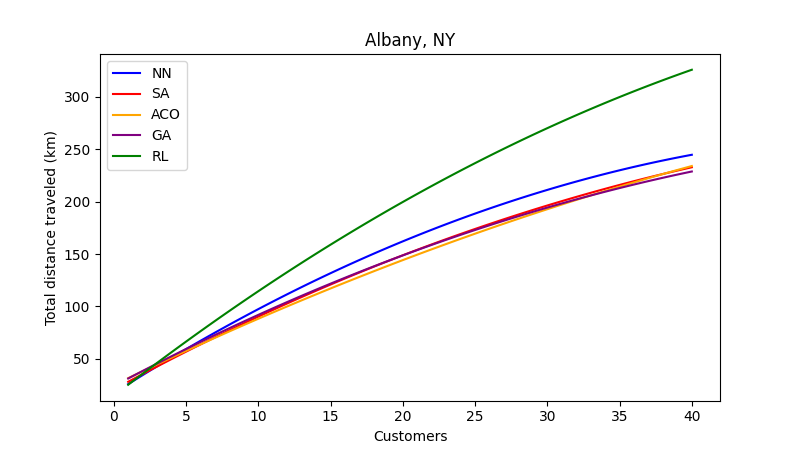
\includegraphics[width=\linewidth]{../data/albany10/comparison.png}
    \caption{Results from PARS executed over Albany, NY with a max. TSP size of 10 customers per truck.}
\end{figure}

\begin{figure}[h]
    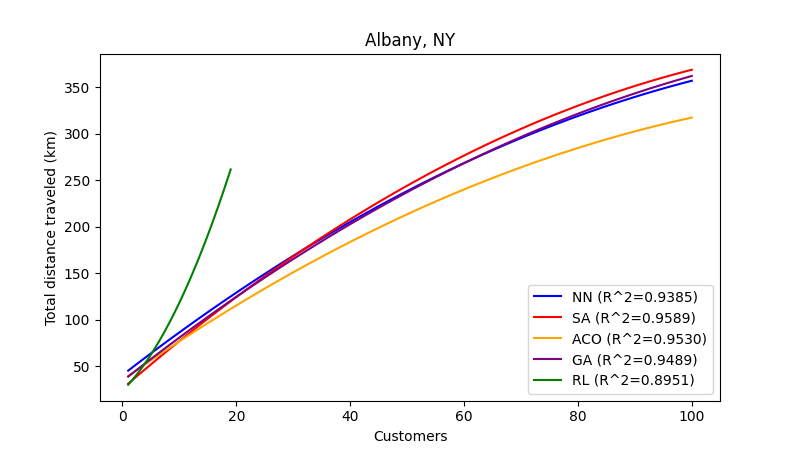
\includegraphics[width=\linewidth]{../data/albany25/comparison.png}
    \caption{Results from PARS executed over Albany, NY with a max. TSP size of 25 customers per truck.}
\end{figure}

\begin{figure}[h]
    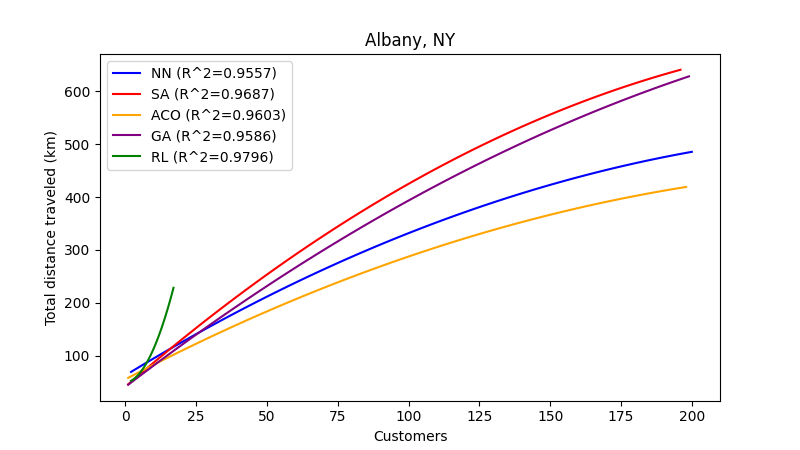
\includegraphics[width=\linewidth]{../data/albany50/comparison.png}
    \caption{Results from PARS executed over Albany, NY with a max. TSP size of 50 customers per truck.}
\end{figure}

\begin{figure}[h]
    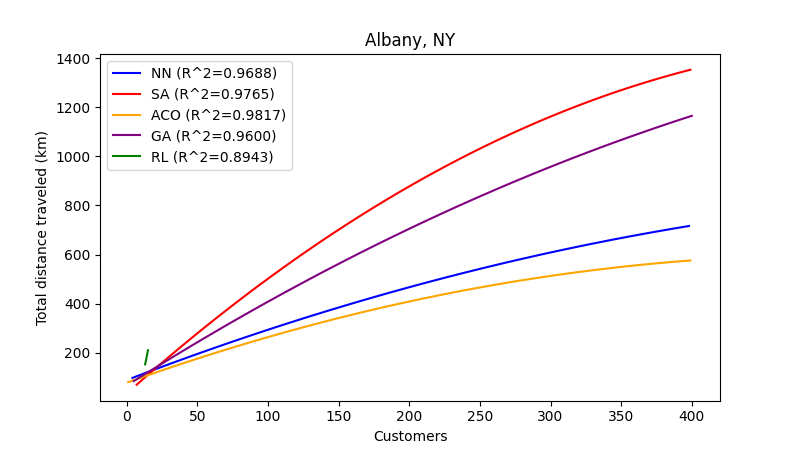
\includegraphics[width=\linewidth]{../data/albany100/comparison.png}
    \caption{Results from PARS executed over Albany, NY with a max. TSP size of 100 customers per truck.}
\end{figure}

\section{Conclusion}

For very small TSP sizes, most algorithms perform better than our baseline with most finding the likely optimal solution. However, as the TSP size is increased, we see a significant divergence. Most notably, ACO performed significantly better than our NN baseline. This is likely because ACO is a more sophisticated algorithm that takes into account both the distance and the pheromone levels, which allows it to find better routes. On the other hand, we noted that once TSP size increased past approximately 10--15, SA, GA and RL performed worse than our NN baseline.

Our baseline, NN, performed relatively well across a broad spectrum of TSP sizes. One reason for this is that the TSP sizes we tested on were relatively small, with the largest being 100 customers. For larger TSP sizes, NN would likely perform much worse as it is a greedy algorithm that does not consider the overall route performance. On the other hand, we also think the map itself may have contributed to the good performance of NN. The map we used was a small, suburban area with a relatively uniform distribution of customers. In such a scenario, NN is more likely to perform well as the nearest neighbor is often a good choice. In contrast, if we were to test on a larger map with a more complex road network and a more clustered distribution of customers, we would likely see a significant drop in the performance of NN.

The randomized nature of SA and GA is likely the reason they performed so poorly on large TSP sizes. For instance, simulated annealing relies on a decay rate. Making the temperature decay happen slower might result in higher-quality solutions. However, we also recognize that our implementations of SA, GA, and RL are very primitive. Moving forward, many of our approaches would require further optimization to out-preform the baseline.

As for RL, we can conclude our findings didn't match that of \cite{Bello2017}. In hindsight, applying RL to VRP is challenging as the state space is very large and the reward structure is complex. The AI needs to learn not only how to find the shortest path but also how to manage multiple trucks and their capacities, which adds an additional layer of complexity. Moreover, the training process for RL can be time-consuming and computationally expensive, especially when dealing with larger maps and more customers. Additionally, our implementation of RL was quite basic, and we may not have tuned the hyperparameters effectively or provided enough training iterations for the model to learn effectively. In contrast,

All-in-all, while RL has shown promise in solving combinatorial optimization problems like TSP and VRP in some research, it is not a guaranteed solution and requires careful design and tuning to achieve good performance.

\bibliographystyle{IEEEtran}
\bibliography{paper}

\end{document}
